\documentclass[11pt,a4paper]{article}
\usepackage[margin=23mm]{geometry}
\usepackage[T1]{fontenc}
\usepackage{lmodern}
\usepackage{amsmath,amssymb,booktabs,array,graphicx,xcolor}
\usepackage[colorlinks=true,linkcolor=blue!50!black,urlcolor=blue!60!black]{hyperref}
\usepackage{fancyhdr}
\definecolor{ink}{HTML}{15364A}
\definecolor{pale}{HTML}{EDF3F7}
\pagestyle{fancy}
\fancyhf{}
\fancyhead[L]{\small Understanding and fitting MCT inflation}
\fancyhead[R]{\small A statistical guide}
\fancyfoot[C]{\thepage}
\setlength{\headheight}{14pt}
\setlength{\parindent}{0pt}
\setlength{\parskip}{6pt}
\setlength{\emergencystretch}{2em}
\newcommand{\E}{\mathbb E}
\newcommand{\Var}{\operatorname{Var}}
\newcommand{\Cov}{\operatorname{Cov}}
\newcommand{\N}{\mathcal N}
\newcommand{\diag}{\operatorname{diag}}
\newcommand{\IG}{\operatorname{IG}}
\newcommand{\takeaway}[1]{\par\medskip\noindent\colorbox{pale}{\parbox{\dimexpr\linewidth-2\fboxsep}{\textbf{Key idea.} #1}}\par\medskip}
\hypersetup{pdftitle={Understanding and Fitting the New York Fed MCT Inflation Model},pdfauthor={Prepared for Michael},pdfsubject={Factor models, state space, and Bayesian estimation}}
\begin{document}
\hypersetup{pageanchor=false}
\begin{titlepage}
\vspace*{18mm}
{\color{ink}\Huge\bfseries Understanding and fitting the New York Fed MCT inflation model\par}
\vspace{9mm}
{\Large From regression to latent factors, state space, and Bayesian sampling\par}
\vspace{10mm}
\textbf{Written for a reader with substantial statistical experience who is new to factor models.}

The central problem is to infer a persistent inflation signal from many noisy sectoral inflation series. The signal is not observed, its relationship with each sector can change, and the noise itself changes over time. This guide explains how the model expresses that problem and how its estimation algorithm solves it in blocks.

\takeaway{A factor is an unobserved regressor shared by several observed series. A loading is the coefficient linking a series to that factor. Neither is the expenditure weight used to aggregate inflation.}

\textbf{Scope.} The mathematical target is the monthly, 17-sector configuration selected by the NY Fed's publicly released PCE replication code: three moving-average lags, no time aggregation, and no extra cross-dependent sector pairs. Sources are linked at the end. This is an explanatory document prepared for this project, not a NY Fed publication.

\textbf{Status distinction.} The Python implementation has passed selected matrix and Gaussian-smoother comparisons against the published code. These checks do not establish convergence of the full Bayesian fit or an exact replication of published MCT estimates. The newer-data reconstruction also has a documented housing-input approximation.

\vfill
{\large Prepared 19 September 2026\par}
\end{titlepage}
\hypersetup{pageanchor=true}
\tableofcontents
\newpage

\section{A factor model is a regression with missing regressors}
Suppose you observe inflation in three sectors. If an economy-wide inflation pressure $f_t$ were observed, you could write three familiar regressions:
\[
y_{1t}=\mu_1+\lambda_1 f_t+e_{1t},\qquad
y_{2t}=\mu_2+\lambda_2 f_t+e_{2t},\qquad
y_{3t}=\mu_3+\lambda_3 f_t+e_{3t}.
\]
The factor-model step is to admit that $f_t$ is \emph{not} observed. You jointly infer its values and the coefficients $\lambda_i$ from the co-movement of the observed series. In vector form, a static Gaussian model is
\begin{equation}
\mathbf y_t=\boldsymbol\mu+\boldsymbol\lambda f_t+\mathbf e_t,
\quad f_t\sim\N(0,1),\quad \mathbf e_t\sim\N(0,\Psi),
\label{eq:static}
\end{equation}
where $\Psi$ is diagonal in the basic version and factor and errors are independent. Consequently,
\[
\Cov(\mathbf y_t)=\boldsymbol\lambda\boldsymbol\lambda'+\Psi.
\]
The shared factor explains off-diagonal covariance; sector-specific errors explain additional variation within individual series. With $k$ factors, replace $\boldsymbol\lambda f_t$ by $\Lambda\mathbf f_t$, where $\Lambda$ is $n\times k$.

\textbf{What does ``extracting a factor'' mean mathematically?} Conditional on known loadings and $\Psi$, the posterior for the single factor in \eqref{eq:static} is
\[
f_t\mid\mathbf y_t\sim\N(m_t,V),\quad
V=(1+\boldsymbol\lambda'\Psi^{-1}\boldsymbol\lambda)^{-1},\quad
m_t=V\boldsymbol\lambda'\Psi^{-1}(\mathbf y_t-\boldsymbol\mu).
\]
This follows by completing the square in the Gaussian likelihood times the $\N(0,1)$ prior. It is a precision-weighted combination of the sector readings. For example, if $\boldsymbol\lambda=(1,1)'$, $\Psi=\diag(1,4)$ and demeaned readings are $(2,4)'$, then $V=1/2.25$ and $m_t=3/2.25=1.33$. The noisier second reading receives less influence, and the prior shrinks the result toward zero.

Conversely, if the factor path were known, estimating each loading would look like regression. Alternating these conditional problems is one route to joint estimation. Dynamic models add information from neighbouring dates.

\textbf{A factor is not automatically an economic cause.} Shared movements can support a common statistical factor without uniquely identifying demand, monetary policy, or supply shocks. Such causal labels require additional identification assumptions.
\takeaway{The factor is learned from the data's shared variation. It is not an externally observed index that gets inserted into an ordinary regression.}

\newpage
\section{Factor, loading, weight: three different objects}
\begin{center}
\begin{tabular}{p{.18\linewidth}p{.31\linewidth}p{.40\linewidth}}
\toprule
Object & Mathematical role & Interpretation\\\midrule
Factor $f_t$ & Shared unobserved regressor & A common pattern across sectors.\\
Loading $\lambda_i$ & Coefficient in $y_{it}=\lambda_i f_t+\cdots$ & The sector's sensitivity to that pattern.\\
Weight $w_{it}$ & Coefficient in a final aggregation & The sector's share of core expenditure.\\\bottomrule
\end{tabular}
\end{center}
Loadings do not need to sum to one and can have either sign. Core expenditure weights do sum to one. A large sector need not have a high loading, and a small sector may provide valuable information about the factor if it is informative and relatively quiet.

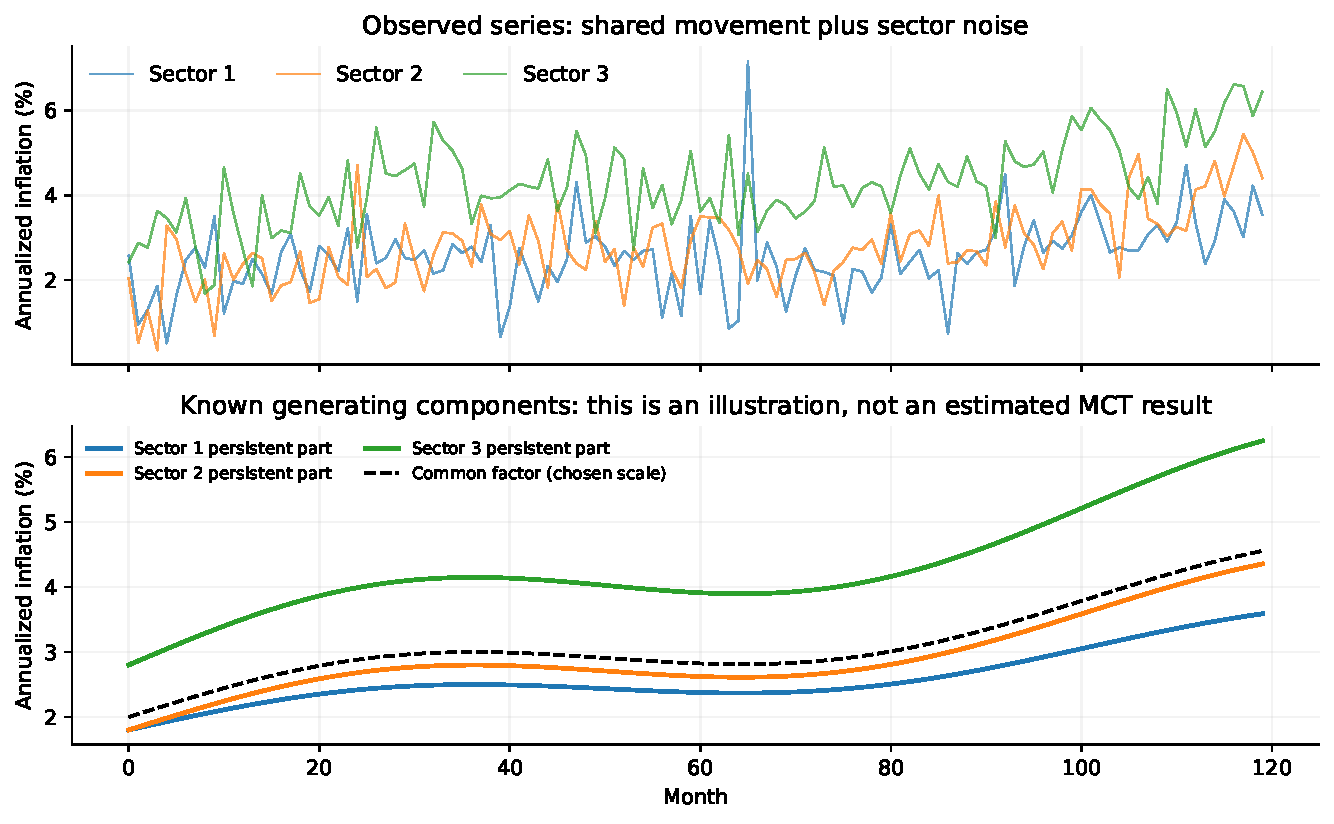
\includegraphics[width=\linewidth]{factor_illustration.pdf}

The figure is generated from invented data with known components. The first sector has a large isolated spike, but all three share a gradual rise. A fitted model must infer these components; it does not get to observe the smooth lines shown in the lower panel.

\textbf{Identification matters.} The products are unchanged if you multiply $f_t$ by $c$ and divide every loading by $c$. The sign can also flip. Static models often fix $\Var(f_t)=1$ and choose a sign convention. With several factors, rotations introduce additional ambiguity. For MCT, interpret sector products and the aggregate rather than treating the raw common factor's level as the national inflation rate. The published code also warns that the allocation of levels between common and sector-specific trends is not identified without normalizations.

\newpage
\section{How PCA, factor models, and state space fit together}
PCA finds linear combinations that explain maximal observed variance. A probabilistic factor model specifies how latent variables generate observed data, including a model for residual variance. Their solutions coincide only under particular assumptions. In particular, the first principal component need not be persistent inflation: a large common temporary shock can dominate observed variance.

To introduce time, let a factor evolve according to an equation such as
\[
f_t=\rho f_{t-1}+\eta_t,\qquad \eta_t\sim\N(0,q).
\]
Now nearby observations help identify the factor. This is a \emph{dynamic} factor model. It is also a state-space model:
\begin{align*}
\mathbf y_t&=Z\mathbf x_t+\boldsymbol\epsilon_t
&&\text{observation equation},\\
\mathbf x_{t+1}&=F\mathbf x_t+G\boldsymbol\eta_t
&&\text{transition equation}.
\end{align*}
The state $\mathbf x_t$ contains the factor and any other hidden quantities needed to explain the data.

\begin{center}
\begin{tabular}{p{.22\linewidth}p{.67\linewidth}}
\toprule
Term & What it tells you\\\midrule
Factor model & Some latent influences are shared across observed series.\\
State-space model & Hidden states evolve through time and generate observations.\\
Bayesian estimation & Unknown states and parameters receive a posterior distribution.\\
Kalman filter & Computes conditional Gaussian updates given the state-space matrices.\\
MCMC & Samples the joint posterior when the whole model cannot be solved in one Gaussian calculation.\\\bottomrule
\end{tabular}
\end{center}

These terms describe different aspects of the same model. A state-space model need not contain a common factor. A factor model need not be dynamic or Bayesian. The MCT model is all three.

\textbf{Connection with VARs.} A VAR models observed variables using their observed lags. A dynamic factor model can instead put a VAR on a small set of hidden factors and connect them to many observed series. MCT uses random-walk trend states and finite-memory transitory components rather than simply fitting an unrestricted VAR to the 17 observed inflation series.
\takeaway{MCT estimates persistence explicitly. Maximising explained cross-sectional variance alone would not distinguish persistent pressure from temporary co-movement.}

\newpage
\section{The actual MCT model: what generates sector inflation?}
Let $i=1,\ldots,17$ index sectors and $t$ index months. A compact representation of the published monthly configuration is
\begin{equation}
y_{it}=a_{it}\tau_{ct}+\tau_{it}+b_{it}e_{ct}
       +e_{it}+\sum_{\ell=1}^{3}\theta_{i\ell}e_{i,t-\ell}+\delta_{it}.
\label{eq:mct}
\end{equation}
Here $\delta_{it}\sim\N(0,10^{-6})$ is the small observation variance used in the code. The substantive decomposition is:
\begin{center}
\begin{tabular}{p{.35\linewidth}p{.54\linewidth}}
\toprule
Component & Meaning\\\midrule
$a_{it}\tau_{ct}$ & Common persistent influence, scaled for sector $i$.\\
$\tau_{it}$ & Additional persistent movement specific to sector $i$.\\
$b_{it}e_{ct}$ & Common transitory influence, scaled for sector $i$.\\
$e_{it}+\sum_{\ell=1}^{3}\theta_{i\ell}e_{i,t-\ell}$ & Sector-specific transitory component with MA(3) dynamics.\\\bottomrule
\end{tabular}
\end{center}
The two trends and the two loading paths evolve as
\begin{align}
\tau_{ct}&=\tau_{c,t-1}+\sigma_{\Delta\tau,c,t}z_{\Delta\tau,c,t},\\
\tau_{it}&=\tau_{i,t-1}+\sigma_{\Delta\tau,i,t}z_{\Delta\tau,i,t},\\
a_{it}&=a_{i,t-1}+\lambda_{a,i}z_{a,i,t},\qquad
b_{it}=b_{i,t-1}+\lambda_{b,i}z_{b,i,t}.
\end{align}
Innovations $z$ are standard normal and independent across their basic innovation channels. Dependence among sectors arises through the shared components. The $\lambda$ parameters govern the smoothness of the loadings; they are estimated rather than re-estimated independently at every date.

\textbf{Why call the first two terms persistent?} An innovation to a random-walk trend remains in its level unless subsequent innovations offset it. In contrast, a sector transitory innovation enters the observation for at most four months through the MA(3) term. ``Transitory'' therefore does not mean ``lasts only one month.''

The sector's persistent inflation is
\[g_{it}=a_{it}\tau_{ct}+\tau_{it}.\]
Removing sector-specific trends would change the target: MCT is not just the common factor. The model estimates two shared channels---persistent and transitory---alongside sector-specific channels. Sources: \cite{nyfed,code}.

\newpage
\section{Changing volatility and outliers are different mechanisms}
For the common and sector-specific transitory innovations, the code uses
\[
e_{jt}=r_{jt}\sigma_{e,j,t}z_{e,j,t},\qquad j\in\{c,1,\ldots,17\}.
\]
The ordinary shock scale is $\sigma_{e,j,t}$. The multiplier $r_{jt}$ allows an occasional outlier. Its support is $\{1\}\cup\{39\text{ equally spaced values from }2\text{ to }10\}$. If $p_j$ denotes the probability of an ordinary observation,
\[
\Pr(r_{jt}=1)=p_j,\qquad
\Pr(r_{jt}=r)=\frac{1-p_j}{39}\quad(r>1).
\]
A large observation can then be explained partly by a transitory outlier without forcing a comparably large trend revision. It is not automatically labelled an outlier; that allocation is inferred jointly with everything else.

For each trend-innovation or transitory-innovation scale, log variance follows a random walk:
\[
h_{jt}=\log\sigma_{jt}^2,\qquad
h_{jt}=h_{j,t-1}+\gamma_j u_{jt},\quad u_{jt}\sim\N(0,1).
\]
There are $2(17+1)=36$ such volatility paths. A period of sustained turbulence can raise the ordinary volatility path; an isolated extraordinary observation can instead receive a large $r_{jt}$. The prior and the surrounding data affect that distinction.

\textbf{Why this complicates fitting.} With known variances and loadings, the hidden inflation states are linear Gaussian. But $a_{it}\tau_{ct}$ multiplies two unknown quantities, and $\exp(h_{jt})$ enters a variance. The whole joint problem is not one ordinary Gaussian regression or one Kalman-filter pass.

\textbf{A useful intuition.} A jump in one noisy sector provides weaker evidence for common persistent inflation than a sustained, coherent movement across many relatively quiet sectors. Yet the model does not apply a hard threshold such as ``three rising months equals trend.'' It allocates probabilities across alternative decompositions under its specified dynamics.
\takeaway{The trend is estimated under assumptions about persistence and noise. It is not an observable truth obtained by mechanically smoothing an aggregate.}

\newpage
\section{Data preparation: what goes into the estimator?}
For a seasonally adjusted sector price index $P_{it}$, the supplied replication data use annualized monthly inflation:
\begin{equation}
y_{it}=100\left[\left(\frac{P_{it}}{P_{i,t-1}}\right)^{12}-1\right].
\end{equation}
For a 0.2\% monthly increase, this is $100(1.002^{12}-1)\simeq2.43\%$. It is not the twelve-month change $100(P_{it}/P_{i,t-12}-1)$, although both are reported in annual percentage units. A sudden monthly observation can be large in annualized terms.

The original replication snapshot contains enough earlier observations to construct a sample from January 1960 through October 2023: $T=766$ and $n=17$. The observation matrix is therefore $766\times17$. The newer local reconstruction runs through July 2026 and has 799 estimation months. Index reference bases cancel in price ratios, but rebasing must not introduce an artificial discontinuity within a series.

\textbf{All sectors inform inference; only core sectors enter the reported aggregate.} The supplied core weights exclude three sector rows: food and beverages purchased for off-premises consumption; gasoline and other energy goods; and gas/electric utilities. Food services and accommodation remain included under this definition. For nominal spending $V_{it}$ and included set $\mathcal C$,
\[
w_{it}=\begin{cases}
V_{it}/\sum_{j\in\mathcal C}V_{jt},&i\in\mathcal C,\\
0,&i\notin\mathcal C.
\end{cases}
\qquad \sum_{i=1}^{17}w_{it}=1.
\]
These weights aggregate inferred trends. They are not factor loadings and do not impose the factor-extraction weights. The model is estimated from sector inflation, not from a weighted average supplied as the sole input.

\textbf{Do not standardize inputs casually.} Replacing each series by a z-score changes the units, priors and aggregation unless the full model and transformation back are adjusted consistently. The supplied estimator receives inflation in percentage units.

\textbf{Local data limitation.} The newer input reconstructs housing excluding gas/electric utilities from housing and water/sanitation using a bilateral Fisher chain. The upstream repository omits its original input-preparation script. That reconstruction is explicitly separate from the exact October 2023 input snapshot. Data revisions also mean a current-vintage fit should not be expected to equal the older published series.

\newpage
\section{What is Bayesian about it?}
Let $X$ contain latent trend and transitory states, $A$ the loadings, $H$ log volatilities, $R$ outlier indicators/scales, and $\Theta$ static parameters. The target is a distribution,
\[
p(X,A,H,R,\Theta\mid Y)
\propto p(Y\mid X,A,H,R,\Theta)\,p(X,A,H,R\mid\Theta)\,p(\Theta).
\]
The likelihood rewards explanations that fit the observations. Transition distributions reward plausible evolution through time. Priors constrain quantities that the data may not identify sharply. The result expresses uncertainty about the entire historical decomposition, not only about a few regression coefficients.

The following are actual hyperparameters in the published driver. We define $\IG(\alpha,\beta)$ by density proportional to $v^{-\alpha-1}\exp(-\beta/v)$ for $v>0$.
\begin{center}
\begin{tabular}{p{.31\linewidth}p{.57\linewidth}}
\toprule
Quantity & Prior specification\\\midrule
Loading innovation variance $\lambda^2$ & $\IG(\nu_\lambda/2,\nu_\lambda s_\lambda^2/2)$; $\nu_\lambda=12$, $s_\lambda^2=0.25^2/(60\cdot12)$.\\[3pt]
Log-volatility innovation variance $\gamma^2$ & Same form; $\nu_\gamma=60$, $s_\gamma^2=1/(60\cdot12)$.\\[3pt]
Ordinary-shock probability $p_j$ & $\operatorname{Beta}(117.5,2.5)$, with mean $47/48$.\\[3pt]
MA coefficient proposal & Gaussian regression update with prior precision $\diag(0.1,0.4,0.9)$, followed by the published root transformation.\\\bottomrule
\end{tabular}
\end{center}
The $s^2$ entries are prior scale parameters, not the prior means of the variances. Initial-state distributions also matter: the initial common trend and common transitory state are fixed at zero; sector trend initial variances are 11 and sector MA-state initial variances are 1. Initial loading covariance matrices are given in the appendix.

For intuition, a small loading-innovation variance favours smoother loading paths. The prior mean for $p_j$ favours rare outliers, without requiring their frequency to remain fixed at $1/48$. The observations update these assumptions.
\takeaway{Priors do more than supply starting values. Starting values launch the algorithm; priors remain part of the posterior throughout estimation.}

\newpage
\section{One sampling sweep, step by step}
The published estimator uses a blocked Gibbs-style MCMC procedure. Begin with initial values and an initial draw of the latent states. Then repeat the following sequence; each block conditions on the most recently available values of the others.
\begin{enumerate}
\item \textbf{Draw the loading paths $a_{it},b_{it}$.} Hold common states and sector trends fixed. The remaining observation equation is linear in the loadings. Their random-walk law supplies the transition equation. The code augments this block with sector MA-noise states and uses a simulation smoother, rather than fitting independent regressions at each date.
\item \textbf{Draw loading smoothness parameters $\lambda$.} Use the increments of the newly drawn loading paths and the inverse-gamma update described below.
\item \textbf{Draw trend and transitory states.} Hold loadings, variances, outlier scales and MA coefficients fixed. Equation \eqref{eq:mct} is now linear Gaussian in the state vector. A simulation smoother draws the whole history jointly, including common and sector-specific trends.
\item \textbf{Draw MA coefficients $\theta_i$.} Conditional on the sector innovations, this is a Gaussian regression calculation followed by the source code's root transformation.
\item \textbf{Draw the 36 volatility paths.} Use trend increments and transitory innovations (with their current outlier scales removed). A normal-mixture approximation permits Gaussian state smoothing for log variance.
\item \textbf{Draw volatility smoothness parameters $\gamma$.} Use increments of the newly drawn log-variance paths.
\item \textbf{Draw outlier scales $r_{jt}$.} Compare how well each allowed scale explains the innovation, combining its likelihood with its current prior probability.
\item \textbf{Draw ordinary-shock probabilities $p_j$.} A beta update uses the sampled counts of ordinary and outlier observations.
\end{enumerate}
One sweep produces a revised, mutually conditioned explanation of the data. Repeating sweeps explores alternatives. These draws are not independent bootstrap datasets, and each iteration is not a new month of observed data. The entire observed sample remains fixed during a fit.

The source uses $t_{\mathrm{skip}}=4$ for several parameter updates and treats the first four innovations as missing in volatility/outlier updates. It still uses those months' inflation observations in the state smoother. This is different from deleting four rows from the model.

\newpage
\section{What the Kalman filter and simulation smoother actually do}
For fixed values of the conditioning parameters, write
\[
\mathbf y_t=Z_t\mathbf x_t+\boldsymbol\epsilon_t,\quad
\boldsymbol\epsilon_t\sim\N(0,H_t),\qquad
\mathbf x_t=F_{t-1}\mathbf x_{t-1}+G_{t-1}\boldsymbol\eta_{t-1},\quad
\boldsymbol\eta_{t-1}\sim\N(0,Q_{t-1}).
\]
Given the previous filtered mean $m_{t-1}$ and covariance $C_{t-1}$, the forward filter computes
\begin{align*}
a_t&=F_{t-1}m_{t-1}, & P_t&=F_{t-1}C_{t-1}F_{t-1}'+G_{t-1}Q_{t-1}G_{t-1}',\\
v_t&=\mathbf y_t-Z_ta_t, & S_t&=Z_tP_tZ_t'+H_t,\\
K_t&=P_tZ_t'S_t^{-1}, & m_t&=a_t+K_tv_t,\\
&& C_t&=P_t-K_tS_tK_t'.
\end{align*}
This is a sequence of Gaussian conditioning calculations. The Kalman gain determines how much the new observation changes the prior state prediction, given its uncertainty and the observation's noise.

\textbf{Filtering versus smoothing.} Filtering gives $p(\mathbf x_t\mid Y_{1:t},\Theta)$. Smoothing uses the full sample and gives $p(\mathbf x_t\mid Y_{1:T},\Theta)$. A later observation can therefore change the historical estimate for an earlier month.

\textbf{Smoothing a mean versus drawing a path.} The Gibbs algorithm needs a draw from the joint conditional distribution $p(\mathbf x_{0:T}\mid Y,\Theta)$, not just its mean. Replacing every draw by a mean would discard state uncertainty and would no longer be the same sampler. Nor can one independently draw from each date's marginal distribution: the cross-time covariance matters.

One Gaussian simulation-smoothing construction is:
\begin{enumerate}
\item Generate auxiliary states and observations $(X^+,Y^+)$ under the current model.
\item Smooth the residual observations $Y-Y^+$ under the corresponding zero-mean formulation.
\item Add the smoothed correction to $X^+$.
\end{enumerate}
The resulting path has the required conditional distribution when initial means and covariances are handled consistently. This is the principle behind the upstream simulation smoother. Our Python implementation delegates the general filtering and simulation-smoothing calculations to \texttt{statsmodels}; it assembles the MCT-specific matrices and updates.

\newpage
\section{The other Bayesian updates, in equations}
\textbf{Innovation variances.} Suppose $d_t\mid v\sim\N(0,v)$ and $v\sim\IG(\nu/2,\nu s^2/2)$. With $m$ included increments,
\[
v\mid d\sim\IG\left(\frac{\nu+m}{2},\frac{\nu s^2+\sum_t d_t^2}{2}\right).
\]
This is used for loading-increment variances and log-volatility-increment variances. The code returns a standard deviation, $\sqrt v$, after drawing the variance through a reciprocal gamma calculation.

\textbf{MA coefficients.} For the rescaled conditional regression $\widetilde{\mathbf u}=X\boldsymbol\theta+\boldsymbol\varepsilon$ with unit error variance and zero-mean prior precision $P$,
\[
V_\theta=(P+X'X)^{-1},\quad m_\theta=V_\theta X'\widetilde{\mathbf u},\quad
\boldsymbol\theta^*\sim\N(m_\theta,V_\theta).
\]
The upstream code uses a pseudoinverse and then transforms polynomial roots to enforce its MA convention. Thus the final update is not merely an unconstrained normal draw; the port reproduces that particular transformation. It should not be described as generic rejection sampling from a truncated Gaussian posterior.

\textbf{Outlier allocations.} For standardized innovation $x_t=e_t/\sigma_t$ and candidate multiplier $r_k$,
\[
\Pr(r_t=r_k\mid x_t,\cdots)\propto
\Pr(r_t=r_k)\frac{1}{r_k}\exp\left(-\frac{x_t^2}{2r_k^2}\right).
\]
If $n_1$ sampled scales equal 1 and $n_o$ exceed 1, then
\[p\mid R\sim\operatorname{Beta}(117.5+n_1,\,2.5+n_o).\]

\textbf{Stochastic volatility.} For $x_t=\sigma_t z_t$, taking log squares gives approximately
\[
\log(x_t^2+10^{-3})=h_t+\log z_t^2.
\]
The log-$\chi^2_1$ error is non-Gaussian. The code approximates it using ten normal mixture components with fixed probabilities, means and variances (following Omori et al.). Conditional on sampled mixture labels, subtract the selected means and use their variances as observation noise. The log-variance random walk then becomes a Gaussian state-space problem. This mixture approximation and the small logarithm offset are part of the implemented algorithm; the procedure is not an exact closed-form solution to the full nonlinear model.

\newpage
\section{Turn posterior draws into the reported inflation measure}
For retained draw $s$, compute sector trends and their aggregate:
\[
g_{it}^{(s)}=a_{it}^{(s)}\tau_{ct}^{(s)}+\tau_{it}^{(s)},\qquad
M_t^{(s)}=\sum_i w_{it}g_{it}^{(s)}.
\]
The reported estimate is the median of $\{M_t^{(s)}\}_s$. The supplied code uses quantiles $1/6$ and $5/6$ for an interval containing $2/3$ of posterior mass; website descriptions round the band to approximately 68\%. The posterior includes uncertainty about states and parameters, conditional on the chosen model and data vintage. It does not automatically include uncertainty over all possible alternative models.

\textbf{A one-month, one-draw example.} Suppose there are three included sectors with weights $(0.5,0.3,0.2)$. Let $\tau_c=2$, loadings $(1,0.8,1.2)$ and sector trends $(0.4,-0.1,0.2)$. Then
\[
\mathbf g=(2.4,1.5,2.6)',\qquad
M=0.5(2.4)+0.3(1.5)+0.2(2.6)=2.17\%.
\]
The common contribution is $2[0.5(1)+0.3(0.8)+0.2(1.2)]=1.96$ percentage points; the specific contribution is $0.5(0.4)+0.3(-0.1)+0.2(0.2)=0.21$. Temporary innovations do not enter this aggregate.

Repeat this calculation for every draw. \textbf{Aggregate first, then take posterior quantiles.} In general,
\[
\operatorname{median}\!\left(\sum_i w_i g_i\right)
\ne \sum_i w_i\operatorname{median}(g_i).
\]
This is why displayed sector contribution medians need not add exactly to the aggregate median. Draw-level contributions do add exactly.

\textbf{Normalization.} The original driver rescales the common trend and its loadings after sampling: $a_{it}^*=a_{it}\sigma_{\Delta\tau,c,t}$ and $\tau_{ct}^*=\tau_{ct}/\sigma_{\Delta\tau,c,t}$. Their product is unchanged, so the Python aggregate can use the unnormalized products. This is a reporting transformation; one should not assume the transformed factor retains the original random-walk transition equation unchanged.

\textbf{Trend versus forecast.} MCT is an inferred persistent component. It is not automatically the forecast of next month's headline inflation. Forecasting requires propagating posterior states and parameter uncertainty forward, adding the transitory dynamics, and specifying future aggregation weights as appropriate.

\newpage
\section{Convergence, validation, and computational cost}
The published driver sets 3,000 burn-in outer iterations, 3,000 retained draws, and two inner sweeps per outer iteration. Its loop also includes iteration zero, so it executes 12,002 sweeps. Burn-in discards the initial portion of the chain to reduce dependence on the starting values; a fixed burn-in length is not proof that this dependence has disappeared. Thinning stores fewer, more widely spaced draws but does not make them independent or guarantee efficient computation.

Each sweep repeatedly processes all months, including two large multivariate state problems and 36 scalar volatility paths. The main state has 87 coordinates and the loading block 102 for the 17-sector MA(3) specification. Thousands of full-history simulation-smoothing calculations explain the hours-long run, despite individual sweeps being fairly quick. The Python implementation is much faster than the initial Octave execution, but it is not claimed to be the fastest possible implementation.

\textbf{What should count as validation?}
\begin{enumerate}
\item Check input definitions, seasonal adjustment, date alignment and expenditure weights. Verify that every month's included weights sum to one.
\item Check state-space matrices and conditional calculations against the source. Our selected initialization/matrix and smoother fixtures pass; this checks components of the implementation.
\item Compare the full October 2023 fit with the NY Fed output using the same data vintage. Numerical differences across seeds and software are expected; quantify them rather than asserting equality.
\item Run multiple chains with different starting points/seeds. Examine trace plots, rank-normalized $\widehat R$, effective sample sizes and Monte Carlo standard errors for the aggregate and other identified quantities. Raw factor signs/scales can obscure diagnostics.
\item Assess sensitivity to priors and influential observations, and inspect posterior predictive behaviour. A narrow interval from a poorly mixed chain is not useful evidence of precision.
\end{enumerate}
The current compact exporter stores aggregate draws and summaries, not every latent parameter draw. More extensive parameter diagnostics require expanding the saved output. Multiple-chain convergence and full replication accuracy remain to be established; the document makes no claim that the running fit has already passed them.

\textbf{Evaluation differs from VAR forecasting.} AIC is not the main validation tool for this latent Bayesian decomposition. If your goal is forecasting, evaluate genuine out-of-sample forecasts using rolling origins, preferably with historical data vintages. Do not use a full-sample smoothed historical MCT as if it had been available in real time: it incorporates later observations and revisions.

\newpage
\appendix
\section{The state vector and an implementation map}
For three MA lags, the main state at $t$ can be ordered as
\[
\mathbf x_t=(\tau_{ct},\tau_{1t},\ldots,\tau_{nt},e_{ct},
e_{1t},e_{1,t-1},e_{1,t-2},e_{1,t-3},\ldots,e_{nt},\ldots,e_{n,t-3})'.
\]
Its dimension is $1+n+1+4n=5n+2=87$. The observation row for sector $i$ picks out its common trend with coefficient $a_{it}$, its own trend with coefficient 1, common noise with coefficient $b_{it}$, and its four noise states with coefficients $(1,\theta_{i1},\theta_{i2},\theta_{i3})$.

The transition matrix retains each trend, resets the new transitory innovations, and shifts each sector's three noise lags down by one position. A selection matrix injects $2(n+1)=36$ independent shocks into the common/sector trends and current transitory innovations. The lagged noise coordinates do not get fresh independent shocks.

The loading block includes $n$ trend loadings, $n$ transitory loadings and $4n$ noise coordinates, for $6n=102$ states. Its observation data are sector inflation minus the currently drawn sector trends. Its time-varying design uses the current common trend and common transitory shock as regressors. The initial loading covariance is $11I_n$ for trend loadings and $I_n+10\mathbf1\mathbf1'$ for transitory loadings; MA-noise initial covariance is $I_{4n}$.

\begin{center}
\begin{tabular}{p{.40\linewidth}p{.49\linewidth}}
\toprule
Local file or object & Role\\\midrule
\texttt{prepare\_inputs.py} & Inflation transformations, dates, sector mapping and normalized weights.\\
\texttt{mct\_python.py: MCT} & Model-specific state matrices and Gibbs update schedule.\\
\texttt{GaussianStates} & Thin adapter to statsmodels simulation smoothing.\\
\texttt{VolatilitySampler} & Mixture allocation and package-based log-volatility smoothing.\\
\texttt{run\_python.py} & Settings, execution, progress and saved draws.\\
\texttt{export\_results.py} & Posterior summaries, reference comparisons and workbooks.\\
\texttt{validate\_python.py} & Source-based matrix/smoother checks.\\
\texttt{upstream/} & Unmodified NY Fed reference source and snapshot.\\\bottomrule
\end{tabular}
\end{center}
In the original code, $a,b$ are \texttt{alpha\_tau, alpha\_eps}; $\tau_c,\tau_i$ are \texttt{tau\_c,tau\_i}; $e_c,e_i$ are \texttt{eps\_c,eps\_i}; and $r$ is \texttt{s\_eps}. The original \texttt{SSM.H} is the observation design matrix; it is called \texttt{design} in statsmodels and $Z_t$ in this guide. Letter conventions differ between libraries.

\newpage
\section{Reading route and sources}
Start with the NY Fed FAQ for the target of the model. Read the introduction in Section 1 of this guide before the technical papers if factors still feel unfamiliar. Use the published code to resolve exact implementation details: the earlier Stock--Watson paper is foundational, but is not a complete specification of every later NY Fed modification.

The code used as reference in this project is pinned to commit:\par
{\small\texttt{7e68e46e2ff4ad55b712f2c6c49f08f9c48e1ea1}}\par
Local copies of the research material are in \texttt{../references/} relative to this document's directory.

\begin{thebibliography}{9}
\bibitem{nyfed} Federal Reserve Bank of New York. \emph{Multivariate Core Trend Inflation: overview and FAQ}. \href{https://www.newyorkfed.org/research/policy/mct}{Open model description}.
\bibitem{code} Federal Reserve Bank of New York, Time Series Analysis Team. \emph{MCT-PCE replication code}. \href{https://github.com/MCT-Inflation-NYFed/MCT-PCE}{Open repository}. In particular: \texttt{automated\_PCE.m}, \texttt{estimate\_MCT.m}, \texttt{update\_vol.m}, \texttt{update\_gam.m}, \texttt{update\_theta.m}, \texttt{update\_scl.m}, and \texttt{update\_ps.m}.
\bibitem{almuzara} Almuzara, M., and A. M. Sbordone (2024). \emph{Measurement and Theory of Core Inflation}. NY Fed Staff Report 1115. \href{https://www.newyorkfed.org/medialibrary/media/research/staff_reports/sr1115.pdf}{Open PDF}.
\bibitem{sw} Stock, J. H., and M. W. Watson (2016). \emph{Core Inflation and Trend Inflation}. Review of Economics and Statistics, 98(4), 770--784. \href{https://www.princeton.edu/~mwatson/papers/core_and_trend_inflation_restat_2016.pdf}{Open paper}; \href{https://www.princeton.edu/~mwatson/papers/core_and_trend_inflation_online_appendix_20151103.pdf}{open technical appendix}.
\bibitem{intro} Almuzara, M., and A. M. Sbordone (2022). \emph{Inflation Persistence: How Much Is There and Where Is It Coming From?} Liberty Street Economics. \href{https://libertystreeteconomics.newyorkfed.org/2022/04/inflation-persistence-how-much-is-there-and-where-is-it-coming-from/}{Open introduction}.
\bibitem{sm} Statsmodels. \emph{SimulationSmoother documentation}. \href{https://www.statsmodels.org/stable/generated/statsmodels.tsa.statespace.simulation_smoother.SimulationSmoother.html}{Open package documentation}. Python implementation uses version 0.14.6.
\end{thebibliography}

\takeaway{To understand one iteration, temporarily treat every unknown except one block as known. That block becomes a familiar regression, Gaussian state-space calculation, or conjugate probability update. MCMC connects those conditional calculations into joint inference.}
\end{document}
